\documentclass[1p]{elsarticle_modified}
%\bibliographystyle{elsarticle-num}

%\usepackage[colorlinks]{hyperref}
%\usepackage{abbrmath_seonhwa} %\Abb, \Ascr, \Acal ,\Abf, \Afrak
\usepackage{amsfonts}
\usepackage{amssymb}
\usepackage{amsmath}
\usepackage{amsthm}
\usepackage{scalefnt}
\usepackage{amsbsy}
\usepackage{kotex}
\usepackage{caption}
\usepackage{subfig}
\usepackage{color}
\usepackage{graphicx}
\usepackage{xcolor} %% white, black, red, green, blue, cyan, magenta, yellow
\usepackage{float}
\usepackage{setspace}
\usepackage{hyperref}

\usepackage{tikz}
\usetikzlibrary{arrows}

\usepackage{multirow}
\usepackage{array} % fixed length table
\usepackage{hhline}

%%%%%%%%%%%%%%%%%%%%%
\makeatletter
\renewcommand*\env@matrix[1][\arraystretch]{%
	\edef\arraystretch{#1}%
	\hskip -\arraycolsep
	\let\@ifnextchar\new@ifnextchar
	\array{*\c@MaxMatrixCols c}}
\makeatother %https://tex.stackexchange.com/questions/14071/how-can-i-increase-the-line-spacing-in-a-matrix
%%%%%%%%%%%%%%%

\usepackage[normalem]{ulem}

\newcommand{\msout}[1]{\ifmmode\text{\sout{\ensuremath{#1}}}\else\sout{#1}\fi}
%SOURCE: \msout is \stkout macro in https://tex.stackexchange.com/questions/20609/strikeout-in-math-mode

\newcommand{\cancel}[1]{
	\ifmmode
	{\color{red}\msout{#1}}
	\else
	{\color{red}\sout{#1}}
	\fi
}

\newcommand{\add}[1]{
	{\color{blue}\uwave{#1}}
}

\newcommand{\replace}[2]{
	\ifmmode
	{\color{red}\msout{#1}}{\color{blue}\uwave{#2}}
	\else
	{\color{red}\sout{#1}}{\color{blue}\uwave{#2}}
	\fi
}

\newcommand{\Sol}{\mathcal{S}} %segment
\newcommand{\D}{D} %diagram
\newcommand{\A}{\mathcal{A}} %arc


%%%%%%%%%%%%%%%%%%%%%%%%%%%%%5 test

\def\sl{\operatorname{\textup{SL}}(2,\Cbb)}
\def\psl{\operatorname{\textup{PSL}}(2,\Cbb)}
\def\quan{\mkern 1mu \triangleright \mkern 1mu}

\theoremstyle{definition}
\newtheorem{thm}{Theorem}[section]
\newtheorem{prop}[thm]{Proposition}
\newtheorem{lem}[thm]{Lemma}
\newtheorem{ques}[thm]{Question}
\newtheorem{cor}[thm]{Corollary}
\newtheorem{defn}[thm]{Definition}
\newtheorem{exam}[thm]{Example}
\newtheorem{rmk}[thm]{Remark}
\newtheorem{alg}[thm]{Algorithm}

\newcommand{\I}{\sqrt{-1}}
\begin{document}

%\begin{frontmatter}
%
%\title{Boundary parabolic representations of knots up to 8 crossings}
%
%%% Group authors per affiliation:
%\author{Yunhi Cho} 
%\address{Department of Mathematics, University of Seoul, Seoul, Korea}
%\ead{yhcho@uos.ac.kr}
%
%
%\author{Seonhwa Kim} %\fnref{s_kim}}
%\address{Center for Geometry and Physics, Institute for Basic Science, Pohang, 37673, Korea}
%\ead{ryeona17@ibs.re.kr}
%
%\author{Hyuk Kim}
%\address{Department of Mathematical Sciences, Seoul National University, Seoul 08826, Korea}
%\ead{hyukkim@snu.ac.kr}
%
%\author{Seokbeom Yoon}
%\address{Department of Mathematical Sciences, Seoul National University, Seoul, 08826,  Korea}
%\ead{sbyoon15@snu.ac.kr}
%
%\begin{abstract}
%We find all boundary parabolic representation of knots up to 8 crossings.
%
%\end{abstract}
%\begin{keyword}
%    \MSC[2010] 57M25 
%\end{keyword}
%
%\end{frontmatter}

%\linenumbers
%\tableofcontents
%
\newcommand\colored[1]{\textcolor{white}{\rule[-0.35ex]{0.8em}{1.4ex}}\kern-0.8em\color{red} #1}%
%\newcommand\colored[1]{\textcolor{white}{ #1}\kern-2.17ex	\textcolor{white}{ #1}\kern-1.81ex	\textcolor{white}{ #1}\kern-2.15ex\color{red}#1	}

{\Large $\underline{12n_{0051}~(K12n_{0051})}$}

\setlength{\tabcolsep}{10pt}
\renewcommand{\arraystretch}{1.6}
\vspace{1cm}\begin{tabular}{m{100pt}>{\centering\arraybackslash}m{274pt}}
\multirow{5}{120pt}{
	\centering
	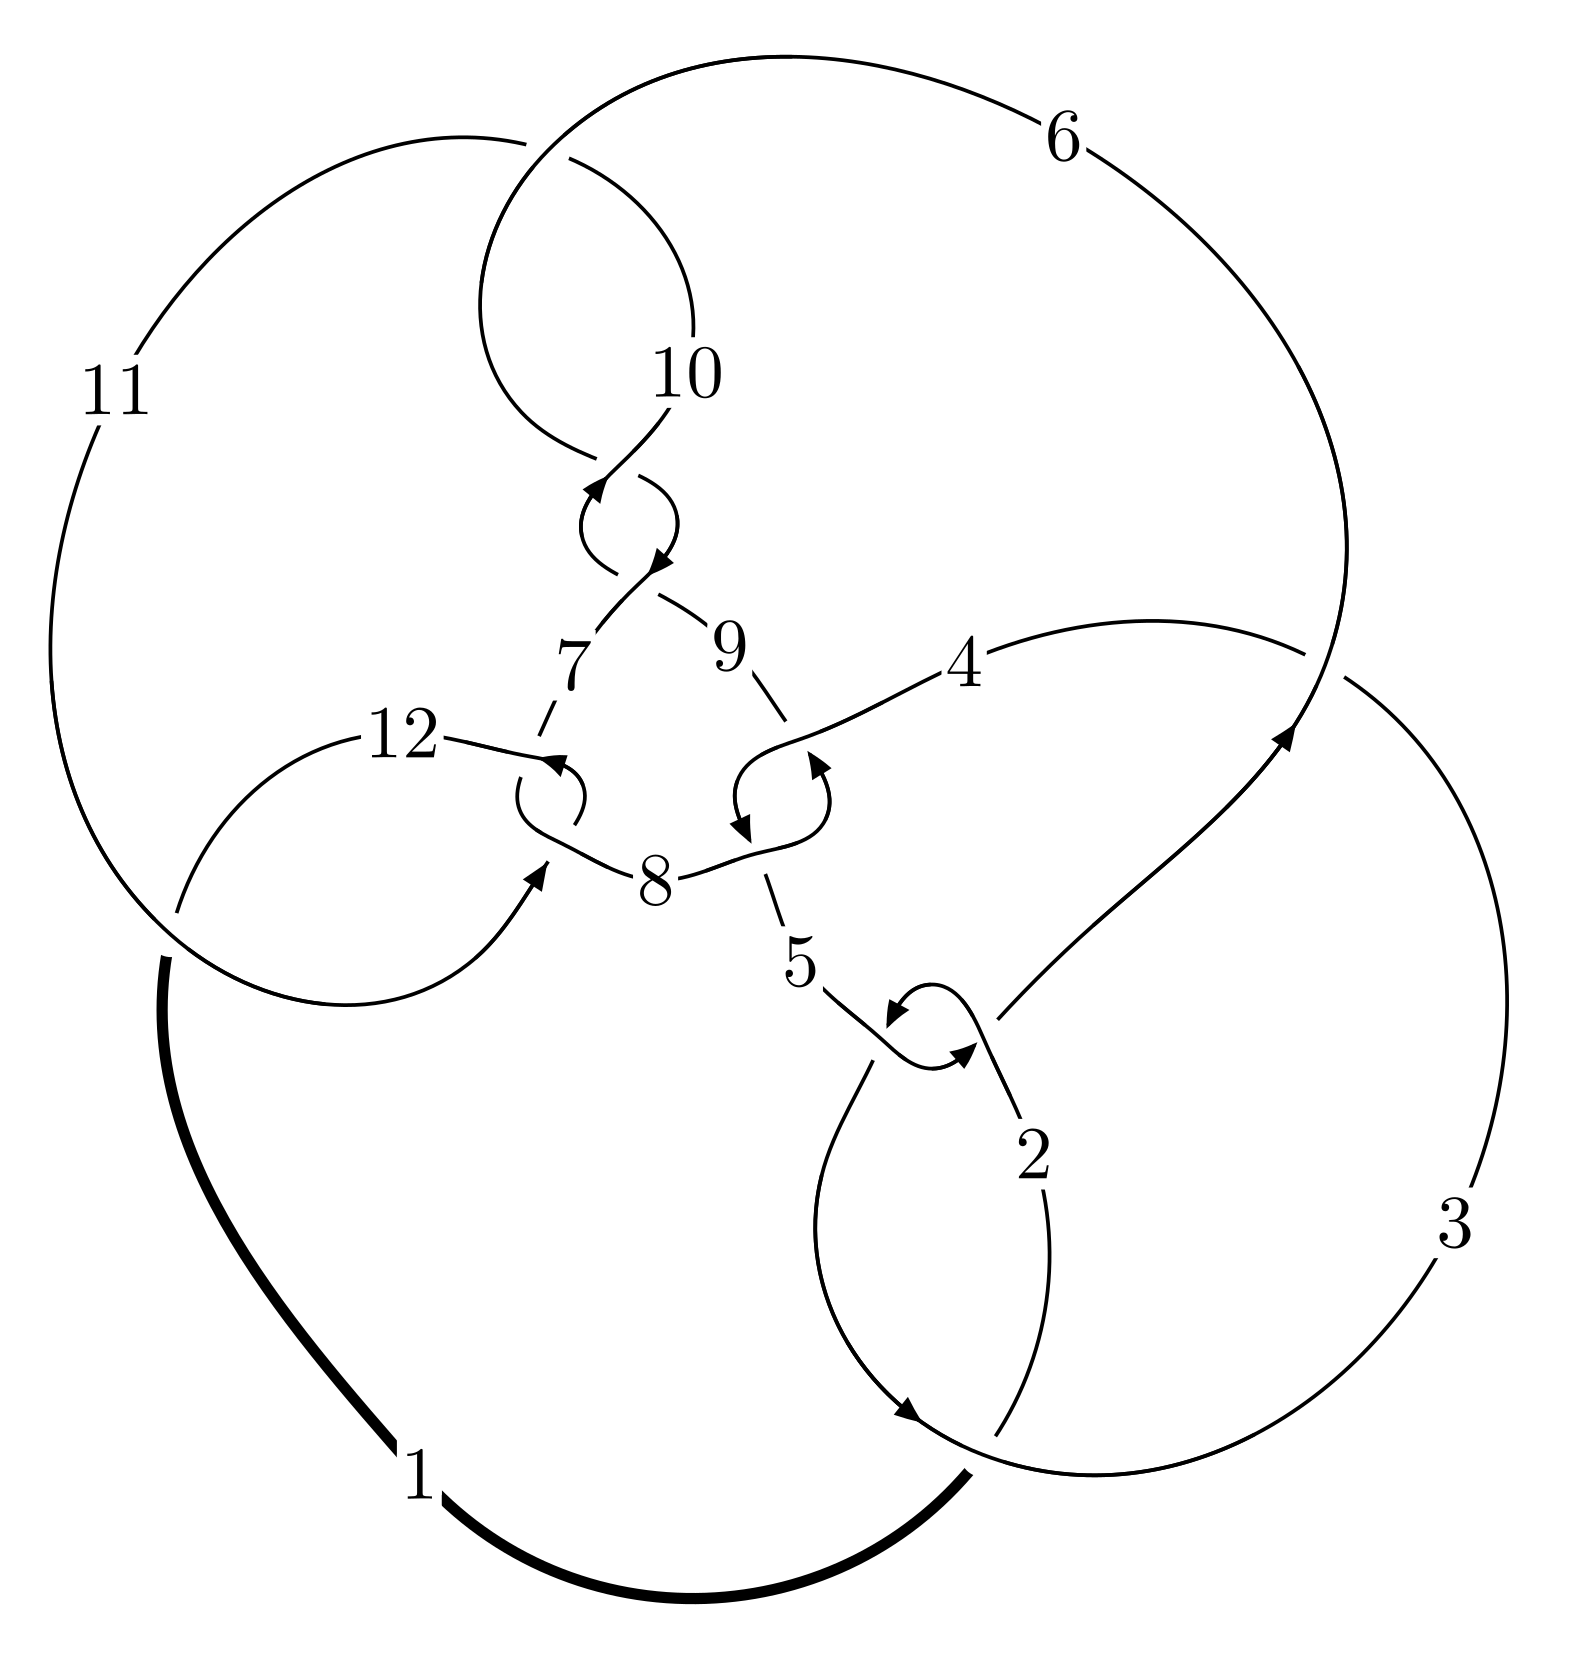
\includegraphics[width=112pt]{../../../GIT/diagram.site/Diagrams/png/2140_12n_0051.png}\\
\ \ \ A knot diagram\footnotemark}&
\allowdisplaybreaks
\textbf{Linearized knot diagam} \\
\cline{2-2}
 &
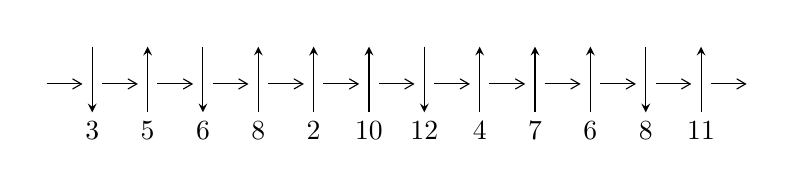
\begin{tikzpicture}[x=20pt, y=17pt]
	% nodes
	\node (C0) at (0, 0) {};
	\node (C1) at (1, 0) {};
	\node (C1U) at (1, +1) {};
	\node (C1D) at (1, -1) {3};

	\node (C2) at (2, 0) {};
	\node (C2U) at (2, +1) {};
	\node (C2D) at (2, -1) {5};

	\node (C3) at (3, 0) {};
	\node (C3U) at (3, +1) {};
	\node (C3D) at (3, -1) {6};

	\node (C4) at (4, 0) {};
	\node (C4U) at (4, +1) {};
	\node (C4D) at (4, -1) {8};

	\node (C5) at (5, 0) {};
	\node (C5U) at (5, +1) {};
	\node (C5D) at (5, -1) {2};

	\node (C6) at (6, 0) {};
	\node (C6U) at (6, +1) {};
	\node (C6D) at (6, -1) {10};

	\node (C7) at (7, 0) {};
	\node (C7U) at (7, +1) {};
	\node (C7D) at (7, -1) {12};

	\node (C8) at (8, 0) {};
	\node (C8U) at (8, +1) {};
	\node (C8D) at (8, -1) {4};

	\node (C9) at (9, 0) {};
	\node (C9U) at (9, +1) {};
	\node (C9D) at (9, -1) {7};

	\node (C10) at (10, 0) {};
	\node (C10U) at (10, +1) {};
	\node (C10D) at (10, -1) {6};

	\node (C11) at (11, 0) {};
	\node (C11U) at (11, +1) {};
	\node (C11D) at (11, -1) {8};

	\node (C12) at (12, 0) {};
	\node (C12U) at (12, +1) {};
	\node (C12D) at (12, -1) {11};
	\node (C13) at (13, 0) {};

	% arrows
	\draw[->,>={angle 60}]
	(C0) edge (C1) (C1) edge (C2) (C2) edge (C3) (C3) edge (C4) (C4) edge (C5) (C5) edge (C6) (C6) edge (C7) (C7) edge (C8) (C8) edge (C9) (C9) edge (C10) (C10) edge (C11) (C11) edge (C12) (C12) edge (C13) ;	\draw[->,>=stealth]
	(C1U) edge (C1D) (C2D) edge (C2U) (C3U) edge (C3D) (C4D) edge (C4U) (C5D) edge (C5U) (C6D) edge (C6U) (C7U) edge (C7D) (C8D) edge (C8U) (C9D) edge (C9U) (C10D) edge (C10U) (C11U) edge (C11D) (C12D) edge (C12U) ;
	\end{tikzpicture} \\
\hhline{~~} \\& 
\textbf{Solving Sequence} \\ \cline{2-2} 
 &
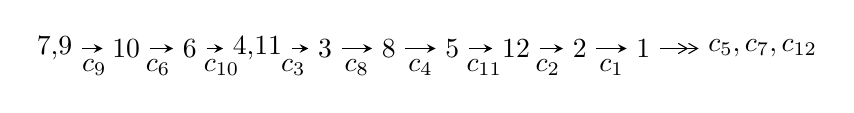
\begin{tikzpicture}[x=23pt, y=7pt]
	% node
	\node (A0) at (-1/8, 0) {7,9};
	\node (A1) at (1, 0) {10};
	\node (A2) at (2, 0) {6};
	\node (A3) at (49/16, 0) {4,11};
	\node (A4) at (33/8, 0) {3};
	\node (A5) at (41/8, 0) {8};
	\node (A6) at (49/8, 0) {5};
	\node (A7) at (57/8, 0) {12};
	\node (A8) at (65/8, 0) {2};
	\node (A9) at (73/8, 0) {1};
	\node (C1) at (1/2, -1) {$c_{9}$};
	\node (C2) at (3/2, -1) {$c_{6}$};
	\node (C3) at (5/2, -1) {$c_{10}$};
	\node (C4) at (29/8, -1) {$c_{3}$};
	\node (C5) at (37/8, -1) {$c_{8}$};
	\node (C6) at (45/8, -1) {$c_{4}$};
	\node (C7) at (53/8, -1) {$c_{11}$};
	\node (C8) at (61/8, -1) {$c_{2}$};
	\node (C9) at (69/8, -1) {$c_{1}$};
	\node (A10) at (11, 0) {$c_{5},c_{7},c_{12}$};

	% edge
	\draw[->,>=stealth]	
	(A0) edge (A1) (A1) edge (A2) (A2) edge (A3) (A3) edge (A4) (A4) edge (A5) (A5) edge (A6) (A6) edge (A7) (A7) edge (A8) (A8) edge (A9) ;
	\draw[->>,>={angle 60}]	
	(A9) edge (A10);
\end{tikzpicture} \\ 

\end{tabular} \\

\footnotetext{
The image of knot diagram is generated by the software ``\textbf{Draw programme}" developed by Andrew Bartholomew(\url{http://www.layer8.co.uk/maths/draw/index.htm\#Running-draw}), where we modified some parts for our purpose(\url{https://github.com/CATsTAILs/LinksPainter}).
}\phantom \\ \newline 
\centering \textbf{Ideals for irreducible components\footnotemark of $X_{\text{par}}$} 
 
\begin{align*}
I^u_{1}&=\langle 
-1.54023\times10^{25} u^{21}-4.36397\times10^{25} u^{20}+\cdots+2.35281\times10^{27} b-1.19412\times10^{26},\\
\phantom{I^u_{1}}&\phantom{= \langle  }4.19615\times10^{28} u^{21}+1.33730\times10^{29} u^{20}+\cdots+1.37404\times10^{30} a+5.83977\times10^{30},\\
\phantom{I^u_{1}}&\phantom{= \langle  }u^{22}+3 u^{21}+\cdots-160 u+73\rangle \\
I^u_{2}&=\langle 
b,\;6 u^3 a-4 u^2 a-3 u^3+4 a^2+14 a u-2 u^2-6 a-7 u-7,\;u^4- u^3+3 u^2-2 u+1\rangle \\
I^u_{3}&=\langle 
- a^4 u+a^3 u+a^3-2 a^2+4 a u+4 b-4 a-4 u,\;a^5+a^4 u- a^4-2 a^3 u-4 a^2 u-4 a^2+4 a-4 u+4,\;u^2+1\rangle \\
\\
\end{align*}
\raggedright * 3 irreducible components of $\dim_{\mathbb{C}}=0$, with total 40 representations.\\
\footnotetext{All coefficients of polynomials are rational numbers. But the coefficients are sometimes approximated in decimal forms when there is not enough margin.}
\newpage
\renewcommand{\arraystretch}{1}
\centering \section*{I. $I^u_{1}= \langle -1.54\times10^{25} u^{21}-4.36\times10^{25} u^{20}+\cdots+2.35\times10^{27} b-1.19\times10^{26},\;4.20\times10^{28} u^{21}+1.34\times10^{29} u^{20}+\cdots+1.37\times10^{30} a+5.84\times10^{30},\;u^{22}+3 u^{21}+\cdots-160 u+73 \rangle$}
\flushleft \textbf{(i) Arc colorings}\\
\begin{tabular}{m{7pt} m{180pt} m{7pt} m{180pt} }
\flushright $a_{7}=$&$\begin{pmatrix}0\\u\end{pmatrix}$ \\
\flushright $a_{9}=$&$\begin{pmatrix}1\\0\end{pmatrix}$ \\
\flushright $a_{10}=$&$\begin{pmatrix}1\\- u^2\end{pmatrix}$ \\
\flushright $a_{6}=$&$\begin{pmatrix}- u\\u^3+u\end{pmatrix}$ \\
\flushright $a_{4}=$&$\begin{pmatrix}-0.0305388 u^{21}-0.0973265 u^{20}+\cdots-6.20155 u-4.25007\\0.00654633 u^{21}+0.0185480 u^{20}+\cdots+4.03131 u+0.0507530\end{pmatrix}$ \\
\flushright $a_{11}=$&$\begin{pmatrix}u^2+1\\- u^4-2 u^2\end{pmatrix}$ \\
\flushright $a_{3}=$&$\begin{pmatrix}-0.0269488 u^{21}-0.0862650 u^{20}+\cdots-5.94433 u-3.75869\\0.00399982 u^{21}+0.0101440 u^{20}+\cdots+3.98951 u-0.419348\end{pmatrix}$ \\
\flushright $a_{8}=$&$\begin{pmatrix}-0.0111557 u^{21}-0.0331545 u^{20}+\cdots-11.4392 u+1.82405\\0.00209278 u^{21}+0.00628667 u^{20}+\cdots+2.38388 u-0.320958\end{pmatrix}$ \\
\flushright $a_{5}=$&$\begin{pmatrix}-0.0325563 u^{21}-0.0995247 u^{20}+\cdots-12.3684 u-1.68756\\0.00662300 u^{21}+0.0176776 u^{20}+\cdots+5.55048 u-0.614116\end{pmatrix}$ \\
\flushright $a_{12}=$&$\begin{pmatrix}0.00503747 u^{21}+0.0176554 u^{20}+\cdots+0.745076 u+3.13839\\-0.000640784 u^{21}-0.00237253 u^{20}+\cdots-0.108742 u-0.457982\end{pmatrix}$ \\
\flushright $a_{2}=$&$\begin{pmatrix}-0.0116342 u^{21}-0.0404516 u^{20}+\cdots+5.25864 u-5.57795\\0.000768008 u^{21}+0.00322339 u^{20}+\cdots+0.588075 u+0.675650\end{pmatrix}$ \\
\flushright $a_{1}=$&$\begin{pmatrix}-0.00471751 u^{21}-0.0164802 u^{20}+\cdots-0.689358 u-2.34200\\0.000443931 u^{21}+0.00178731 u^{20}+\cdots+0.0810747 u+0.491670\end{pmatrix}$\\&\end{tabular}
\flushleft \textbf{(ii) Obstruction class $= -1$}\\~\\
\flushleft \textbf{(iii) Cusp Shapes $= 0.0299967 u^{21}+0.106465 u^{20}+\cdots-19.9627 u+12.9465$}\\~\\
\newpage\renewcommand{\arraystretch}{1}
\flushleft \textbf{(iv) u-Polynomials at the component}\newline \\
\begin{tabular}{m{50pt}|m{274pt}}
Crossings & \hspace{64pt}u-Polynomials at each crossing \\
\hline $$\begin{aligned}c_{1}\end{aligned}$$&$\begin{aligned}
&u^{22}+19 u^{21}+\cdots+79 u+16
\end{aligned}$\\
\hline $$\begin{aligned}c_{2},c_{5}\end{aligned}$$&$\begin{aligned}
&u^{22}+7 u^{21}+\cdots+35 u+4
\end{aligned}$\\
\hline $$\begin{aligned}c_{3}\end{aligned}$$&$\begin{aligned}
&u^{22}-16 u^{21}+\cdots+25000 u+3104
\end{aligned}$\\
\hline $$\begin{aligned}c_{4},c_{8}\end{aligned}$$&$\begin{aligned}
&u^{22}- u^{21}+\cdots+1536 u+2048
\end{aligned}$\\
\hline $$\begin{aligned}c_{6},c_{9},c_{10}\end{aligned}$$&$\begin{aligned}
&u^{22}+3 u^{21}+\cdots-160 u+73
\end{aligned}$\\
\hline $$\begin{aligned}c_{7},c_{11}\end{aligned}$$&$\begin{aligned}
&u^{22}+3 u^{21}+\cdots+182 u+73
\end{aligned}$\\
\hline $$\begin{aligned}c_{12}\end{aligned}$$&$\begin{aligned}
&u^{22}+7 u^{21}+\cdots-67032 u+5329
\end{aligned}$\\
\hline
\end{tabular}\\~\\
\newpage\renewcommand{\arraystretch}{1}
\flushleft \textbf{(v) Riley Polynomials at the component}\newline \\
\begin{tabular}{m{50pt}|m{274pt}}
Crossings & \hspace{64pt}Riley Polynomials at each crossing \\
\hline $$\begin{aligned}c_{1}\end{aligned}$$&$\begin{aligned}
&y^{22}-25 y^{21}+\cdots+179903 y+256
\end{aligned}$\\
\hline $$\begin{aligned}c_{2},c_{5}\end{aligned}$$&$\begin{aligned}
&y^{22}+19 y^{21}+\cdots+79 y+16
\end{aligned}$\\
\hline $$\begin{aligned}c_{3}\end{aligned}$$&$\begin{aligned}
&y^{22}-78 y^{21}+\cdots+78714048 y+9634816
\end{aligned}$\\
\hline $$\begin{aligned}c_{4},c_{8}\end{aligned}$$&$\begin{aligned}
&y^{22}+91 y^{21}+\cdots+30670848 y+4194304
\end{aligned}$\\
\hline $$\begin{aligned}c_{6},c_{9},c_{10}\end{aligned}$$&$\begin{aligned}
&y^{22}+45 y^{21}+\cdots+149016 y+5329
\end{aligned}$\\
\hline $$\begin{aligned}c_{7},c_{11}\end{aligned}$$&$\begin{aligned}
&y^{22}-7 y^{21}+\cdots+67032 y+5329
\end{aligned}$\\
\hline $$\begin{aligned}c_{12}\end{aligned}$$&$\begin{aligned}
&y^{22}+85 y^{21}+\cdots+2794246372 y+28398241
\end{aligned}$\\
\hline
\end{tabular}\\~\\
\newpage\flushleft \textbf{(vi) Complex Volumes and Cusp Shapes}
$$\begin{array}{c|c|c}  
\text{Solutions to }I^u_{1}& \I (\text{vol} + \sqrt{-1}CS) & \text{Cusp shape}\\
 \hline 
\begin{aligned}
u &= \phantom{-}0.166885 + 0.855784 I \\
a &= \phantom{-}0.884204 - 0.564449 I \\
b &= -0.685307 - 0.431142 I\end{aligned}
 & -1.86083 + 1.88410 I & -4.29628 - 4.39442 I \\ \hline\begin{aligned}
u &= \phantom{-}0.166885 - 0.855784 I \\
a &= \phantom{-}0.884204 + 0.564449 I \\
b &= -0.685307 + 0.431142 I\end{aligned}
 & -1.86083 - 1.88410 I & -4.29628 + 4.39442 I \\ \hline\begin{aligned}
u &= \phantom{-}1.245170 + 0.161308 I \\
a &= -0.584895 + 0.469137 I \\
b &= \phantom{-}0.88430 - 1.76284 I\end{aligned}
 & -3.01876 + 2.75600 I & \phantom{-}1.05384 - 1.99167 I \\ \hline\begin{aligned}
u &= \phantom{-}1.245170 - 0.161308 I \\
a &= -0.584895 - 0.469137 I \\
b &= \phantom{-}0.88430 + 1.76284 I\end{aligned}
 & -3.01876 - 2.75600 I & \phantom{-}1.05384 + 1.99167 I \\ \hline\begin{aligned}
u &= \phantom{-}0.065911 + 1.393150 I \\
a &= -0.167886 + 0.219714 I \\
b &= \phantom{-}0.208154 + 0.992360 I\end{aligned}
 & -7.41484 + 5.99413 I & -4.98068 - 7.65331 I \\ \hline\begin{aligned}
u &= \phantom{-}0.065911 - 1.393150 I \\
a &= -0.167886 - 0.219714 I \\
b &= \phantom{-}0.208154 - 0.992360 I\end{aligned}
 & -7.41484 - 5.99413 I & -4.98068 + 7.65331 I \\ \hline\begin{aligned}
u &= -0.147428 + 0.530014 I \\
a &= \phantom{-}2.56324 - 1.19415 I \\
b &= -0.391902 - 0.411319 I\end{aligned}
 & \phantom{-}0.18307 - 2.82080 I & \phantom{-}2.85537 - 1.68871 I \\ \hline\begin{aligned}
u &= -0.147428 - 0.530014 I \\
a &= \phantom{-}2.56324 + 1.19415 I \\
b &= -0.391902 + 0.411319 I\end{aligned}
 & \phantom{-}0.18307 + 2.82080 I & \phantom{-}2.85537 + 1.68871 I \\ \hline\begin{aligned}
u &= \phantom{-}0.309359 + 0.401971 I \\
a &= -0.508079 - 0.818004 I \\
b &= \phantom{-}0.193284 + 0.440196 I\end{aligned}
 & \phantom{-}0.445026 + 1.231770 I & \phantom{-}4.87220 - 5.67709 I \\ \hline\begin{aligned}
u &= \phantom{-}0.309359 - 0.401971 I \\
a &= -0.508079 + 0.818004 I \\
b &= \phantom{-}0.193284 - 0.440196 I\end{aligned}
 & \phantom{-}0.445026 - 1.231770 I & \phantom{-}4.87220 + 5.67709 I\\
 \hline 
 \end{array}$$\newpage$$\begin{array}{c|c|c}  
\text{Solutions to }I^u_{1}& \I (\text{vol} + \sqrt{-1}CS) & \text{Cusp shape}\\
 \hline 
\begin{aligned}
u &= -0.14190 + 1.59059 I \\
a &= -0.104582 - 0.310705 I \\
b &= -0.841835 - 0.832729 I\end{aligned}
 & -5.61868 + 1.54212 I & \phantom{-}1.66178 - 2.03716 I \\ \hline\begin{aligned}
u &= -0.14190 - 1.59059 I \\
a &= -0.104582 + 0.310705 I \\
b &= -0.841835 + 0.832729 I\end{aligned}
 & -5.61868 - 1.54212 I & \phantom{-}1.66178 + 2.03716 I \\ \hline\begin{aligned}
u &= -0.009993 + 0.350116 I \\
a &= -3.01267 - 0.71642 I \\
b &= \phantom{-}0.469397 + 0.461238 I\end{aligned}
 & \phantom{-}0.96093 + 1.37462 I & \phantom{-}8.72525 - 4.65494 I \\ \hline\begin{aligned}
u &= -0.009993 - 0.350116 I \\
a &= -3.01267 + 0.71642 I \\
b &= \phantom{-}0.469397 - 0.461238 I\end{aligned}
 & \phantom{-}0.96093 - 1.37462 I & \phantom{-}8.72525 + 4.65494 I \\ \hline\begin{aligned}
u &= -0.69231 + 1.86047 I \\
a &= -0.585229 - 1.015730 I \\
b &= \phantom{-}1.41273 - 1.99234 I\end{aligned}
 & \phantom{-}15.9166 - 13.0727 I & \phantom{-}0.81219 + 5.19676 I \\ \hline\begin{aligned}
u &= -0.69231 - 1.86047 I \\
a &= -0.585229 + 1.015730 I \\
b &= \phantom{-}1.41273 + 1.99234 I\end{aligned}
 & \phantom{-}15.9166 + 13.0727 I & \phantom{-}0.81219 - 5.19676 I \\ \hline\begin{aligned}
u &= -0.61577 + 2.17742 I \\
a &= \phantom{-}0.394124 + 0.984688 I \\
b &= -1.03067 + 2.69186 I\end{aligned}
 & \phantom{-}19.2619 - 5.9056 I & \phantom{-}2.16347 + 1.69823 I \\ \hline\begin{aligned}
u &= -0.61577 - 2.17742 I \\
a &= \phantom{-}0.394124 - 0.984688 I \\
b &= -1.03067 - 2.69186 I\end{aligned}
 & \phantom{-}19.2619 + 5.9056 I & \phantom{-}2.16347 - 1.69823 I \\ \hline\begin{aligned}
u &= -1.57086 + 2.18266 I \\
a &= \phantom{-}0.515590 + 0.201211 I \\
b &= \phantom{-}1.02473 + 4.03132 I\end{aligned}
 & -13.72130 - 3.06559 I & \phantom{-0.000000 } 0 \\ \hline\begin{aligned}
u &= -1.57086 - 2.18266 I \\
a &= \phantom{-}0.515590 - 0.201211 I \\
b &= \phantom{-}1.02473 - 4.03132 I\end{aligned}
 & -13.72130 + 3.06559 I & \phantom{-0.000000 } 0\\
 \hline 
 \end{array}$$\newpage$$\begin{array}{c|c|c}  
\text{Solutions to }I^u_{1}& \I (\text{vol} + \sqrt{-1}CS) & \text{Cusp shape}\\
 \hline 
\begin{aligned}
u &= -0.10906 + 2.96605 I \\
a &= -0.102719 - 0.793534 I \\
b &= -0.74289 - 4.42273 I\end{aligned}
 & \phantom{-}12.96110 + 1.49730 I & \phantom{-0.000000 } 0 \\ \hline\begin{aligned}
u &= -0.10906 - 2.96605 I \\
a &= -0.102719 + 0.793534 I \\
b &= -0.74289 + 4.42273 I\end{aligned}
 & \phantom{-}12.96110 - 1.49730 I & \phantom{-0.000000 } 0\\
 \hline 
 \end{array}$$\newpage\newpage\renewcommand{\arraystretch}{1}
\centering \section*{II. $I^u_{2}= \langle b,\;6 u^3 a-3 u^3+\cdots-6 a-7,\;u^4- u^3+3 u^2-2 u+1 \rangle$}
\flushleft \textbf{(i) Arc colorings}\\
\begin{tabular}{m{7pt} m{180pt} m{7pt} m{180pt} }
\flushright $a_{7}=$&$\begin{pmatrix}0\\u\end{pmatrix}$ \\
\flushright $a_{9}=$&$\begin{pmatrix}1\\0\end{pmatrix}$ \\
\flushright $a_{10}=$&$\begin{pmatrix}1\\- u^2\end{pmatrix}$ \\
\flushright $a_{6}=$&$\begin{pmatrix}- u\\u^3+u\end{pmatrix}$ \\
\flushright $a_{4}=$&$\begin{pmatrix}a\\0\end{pmatrix}$ \\
\flushright $a_{11}=$&$\begin{pmatrix}u^2+1\\- u^3+u^2-2 u+1\end{pmatrix}$ \\
\flushright $a_{3}=$&$\begin{pmatrix}u^3 a-2 u^2 a+2 a u\\u^3 a-2 u^2 a+a u\end{pmatrix}$ \\
\flushright $a_{8}=$&$\begin{pmatrix}1\\0\end{pmatrix}$ \\
\flushright $a_{5}=$&$\begin{pmatrix}a\\0\end{pmatrix}$ \\
\flushright $a_{12}=$&$\begin{pmatrix}u^3+2 u\\- u^3+u^2-2 u+1\end{pmatrix}$ \\
\flushright $a_{2}=$&$\begin{pmatrix}u^3 a-2 u^2 a+\frac{3}{2} u^3+2 a u- u^2+\frac{7}{2} u-\frac{3}{2}\\u^3 a-2 u^2 a+a u\end{pmatrix}$ \\
\flushright $a_{1}=$&$\begin{pmatrix}u\\- u^3- u\end{pmatrix}$\\&\end{tabular}
\flushleft \textbf{(ii) Obstruction class $= 1$}\\~\\
\flushleft \textbf{(iii) Cusp Shapes $= \frac{9}{2} u^3 a-5 u^2 a-\frac{19}{4} u^3+\frac{21}{2} a u+\frac{7}{2} u^2-\frac{7}{2} a-\frac{55}{4} u+\frac{17}{4}$}\\~\\
\newpage\renewcommand{\arraystretch}{1}
\flushleft \textbf{(iv) u-Polynomials at the component}\newline \\
\begin{tabular}{m{50pt}|m{274pt}}
Crossings & \hspace{64pt}u-Polynomials at each crossing \\
\hline $$\begin{aligned}c_{1},c_{3},c_{5}\end{aligned}$$&$\begin{aligned}
&(u^2- u+1)^4
\end{aligned}$\\
\hline $$\begin{aligned}c_{2}\end{aligned}$$&$\begin{aligned}
&(u^2+u+1)^4
\end{aligned}$\\
\hline $$\begin{aligned}c_{4},c_{8}\end{aligned}$$&$\begin{aligned}
&u^8
\end{aligned}$\\
\hline $$\begin{aligned}c_{6}\end{aligned}$$&$\begin{aligned}
&(u^4+u^3+3 u^2+2 u+1)^2
\end{aligned}$\\
\hline $$\begin{aligned}c_{7}\end{aligned}$$&$\begin{aligned}
&(u^4+u^3+u^2+1)^2
\end{aligned}$\\
\hline $$\begin{aligned}c_{9},c_{10},c_{12}\end{aligned}$$&$\begin{aligned}
&(u^4- u^3+3 u^2-2 u+1)^2
\end{aligned}$\\
\hline $$\begin{aligned}c_{11}\end{aligned}$$&$\begin{aligned}
&(u^4- u^3+u^2+1)^2
\end{aligned}$\\
\hline
\end{tabular}\\~\\
\newpage\renewcommand{\arraystretch}{1}
\flushleft \textbf{(v) Riley Polynomials at the component}\newline \\
\begin{tabular}{m{50pt}|m{274pt}}
Crossings & \hspace{64pt}Riley Polynomials at each crossing \\
\hline $$\begin{aligned}c_{1},c_{2},c_{3}\\c_{5}\end{aligned}$$&$\begin{aligned}
&(y^2+y+1)^4
\end{aligned}$\\
\hline $$\begin{aligned}c_{4},c_{8}\end{aligned}$$&$\begin{aligned}
&y^8
\end{aligned}$\\
\hline $$\begin{aligned}c_{6},c_{9},c_{10}\\c_{12}\end{aligned}$$&$\begin{aligned}
&(y^4+5 y^3+7 y^2+2 y+1)^2
\end{aligned}$\\
\hline $$\begin{aligned}c_{7},c_{11}\end{aligned}$$&$\begin{aligned}
&(y^4+y^3+3 y^2+2 y+1)^2
\end{aligned}$\\
\hline
\end{tabular}\\~\\
\newpage\flushleft \textbf{(vi) Complex Volumes and Cusp Shapes}
$$\begin{array}{c|c|c}  
\text{Solutions to }I^u_{2}& \I (\text{vol} + \sqrt{-1}CS) & \text{Cusp shape}\\
 \hline 
\begin{aligned}
u &= \phantom{-}0.395123 + 0.506844 I \\
a &= -1.13839 - 1.09665 I \\
b &= \phantom{-0.000000 } 0\end{aligned}
 & \phantom{-}0.21101 + 3.44499 I & \phantom{-}3.71851 - 10.46973 I \\ \hline\begin{aligned}
u &= \phantom{-}0.395123 + 0.506844 I \\
a &= \phantom{-}1.51892 - 0.43755 I \\
b &= \phantom{-0.000000 } 0\end{aligned}
 & \phantom{-}0.211005 - 0.614778 I & \phantom{-}1.372162 - 0.328352 I \\ \hline\begin{aligned}
u &= \phantom{-}0.395123 - 0.506844 I \\
a &= -1.13839 + 1.09665 I \\
b &= \phantom{-0.000000 } 0\end{aligned}
 & \phantom{-}0.21101 - 3.44499 I & \phantom{-}3.71851 + 10.46973 I \\ \hline\begin{aligned}
u &= \phantom{-}0.395123 - 0.506844 I \\
a &= \phantom{-}1.51892 + 0.43755 I \\
b &= \phantom{-0.000000 } 0\end{aligned}
 & \phantom{-}0.211005 + 0.614778 I & \phantom{-}1.372162 + 0.328352 I \\ \hline\begin{aligned}
u &= \phantom{-}0.10488 + 1.55249 I \\
a &= -0.435815 + 0.100890 I \\
b &= \phantom{-0.000000 } 0\end{aligned}
 & -6.79074 + 5.19385 I & \phantom{-}0.529613 - 1.243149 I \\ \hline\begin{aligned}
u &= \phantom{-}0.10488 + 1.55249 I \\
a &= \phantom{-}0.305281 + 0.326982 I \\
b &= \phantom{-0.000000 } 0\end{aligned}
 & -6.79074 + 1.13408 I & -4.49529 - 1.20873 I \\ \hline\begin{aligned}
u &= \phantom{-}0.10488 - 1.55249 I \\
a &= -0.435815 - 0.100890 I \\
b &= \phantom{-0.000000 } 0\end{aligned}
 & -6.79074 - 5.19385 I & \phantom{-}0.529613 + 1.243149 I \\ \hline\begin{aligned}
u &= \phantom{-}0.10488 - 1.55249 I \\
a &= \phantom{-}0.305281 - 0.326982 I \\
b &= \phantom{-0.000000 } 0\end{aligned}
 & -6.79074 - 1.13408 I & -4.49529 + 1.20873 I\\
 \hline 
 \end{array}$$\newpage\newpage\renewcommand{\arraystretch}{1}
\centering \section*{III. $I^u_{3}= \langle - a^4 u+a^3 u+\cdots-2 a^2-4 a,\;a^4 u-2 a^3 u+\cdots+4 a+4,\;u^2+1 \rangle$}
\flushleft \textbf{(i) Arc colorings}\\
\begin{tabular}{m{7pt} m{180pt} m{7pt} m{180pt} }
\flushright $a_{7}=$&$\begin{pmatrix}0\\u\end{pmatrix}$ \\
\flushright $a_{9}=$&$\begin{pmatrix}1\\0\end{pmatrix}$ \\
\flushright $a_{10}=$&$\begin{pmatrix}1\\1\end{pmatrix}$ \\
\flushright $a_{6}=$&$\begin{pmatrix}- u\\0\end{pmatrix}$ \\
\flushright $a_{4}=$&$\begin{pmatrix}a\\\frac{1}{4} a^4 u-\frac{1}{4} a^3 u+\cdots+\frac{1}{2} a^2+a\end{pmatrix}$ \\
\flushright $a_{11}=$&$\begin{pmatrix}0\\1\end{pmatrix}$ \\
\flushright $a_{3}=$&$\begin{pmatrix}-\frac{1}{4} a^4 u+\frac{1}{4} a^3 u+\cdots+\frac{1}{4} a^3-\frac{1}{2} a^2\\\frac{1}{4} a^4 u-\frac{1}{4} a^3 u+\cdots+\frac{1}{2} a^2+a\end{pmatrix}$ \\
\flushright $a_{8}=$&$\begin{pmatrix}- u\\-\frac{1}{2} a^3 u+a^2 u+\cdots+\frac{1}{2} a-3\end{pmatrix}$ \\
\flushright $a_{5}=$&$\begin{pmatrix}\frac{1}{4} a^3 u-\frac{1}{2} a^2 u+\cdots-\frac{1}{4} a^3+1\\-\frac{1}{2} a^4 u+\frac{3}{4} a^3 u+\cdots-2 a^2- a\end{pmatrix}$ \\
\flushright $a_{12}=$&$\begin{pmatrix}1\\-\frac{1}{4} a^4 u+\frac{1}{2} a^3 u+\cdots-\frac{1}{2} a+1\end{pmatrix}$ \\
\flushright $a_{2}=$&$\begin{pmatrix}-\frac{1}{2} a^4 u+\frac{1}{4} a^3 u+\cdots-2 a^2-1\\\frac{1}{2} a^4 u-\frac{3}{4} a^3 u+\cdots+2 a^2+\frac{1}{2} a\end{pmatrix}$ \\
\flushright $a_{1}=$&$\begin{pmatrix}1\\-\frac{1}{4} a^4 u+\frac{1}{2} a^3 u+\cdots- a^2-\frac{1}{2} a\end{pmatrix}$\\&\end{tabular}
\flushleft \textbf{(ii) Obstruction class $= 1$}\\~\\
\flushleft \textbf{(iii) Cusp Shapes $= a^4+2 a^3 u-2 a^3-6 a^2 u+8$}\\~\\
\newpage\renewcommand{\arraystretch}{1}
\flushleft \textbf{(iv) u-Polynomials at the component}\newline \\
\begin{tabular}{m{50pt}|m{274pt}}
Crossings & \hspace{64pt}u-Polynomials at each crossing \\
\hline $$\begin{aligned}c_{1}\end{aligned}$$&$\begin{aligned}
&(u^5-3 u^4+4 u^3- u^2- u+1)^2
\end{aligned}$\\
\hline $$\begin{aligned}c_{2}\end{aligned}$$&$\begin{aligned}
&(u^5- u^4+2 u^3- u^2+u-1)^2
\end{aligned}$\\
\hline $$\begin{aligned}c_{3}\end{aligned}$$&$\begin{aligned}
&(u^5+u^4-2 u^3- u^2+u-1)^2
\end{aligned}$\\
\hline $$\begin{aligned}c_{4},c_{8}\end{aligned}$$&$\begin{aligned}
&u^{10}+5 u^8+8 u^6+3 u^4- u^2+1
\end{aligned}$\\
\hline $$\begin{aligned}c_{5}\end{aligned}$$&$\begin{aligned}
&(u^5+u^4+2 u^3+u^2+u+1)^2
\end{aligned}$\\
\hline $$\begin{aligned}c_{6},c_{7},c_{9}\\c_{10},c_{11}\end{aligned}$$&$\begin{aligned}
&(u^2+1)^5
\end{aligned}$\\
\hline $$\begin{aligned}c_{12}\end{aligned}$$&$\begin{aligned}
&(u-1)^{10}
\end{aligned}$\\
\hline
\end{tabular}\\~\\
\newpage\renewcommand{\arraystretch}{1}
\flushleft \textbf{(v) Riley Polynomials at the component}\newline \\
\begin{tabular}{m{50pt}|m{274pt}}
Crossings & \hspace{64pt}Riley Polynomials at each crossing \\
\hline $$\begin{aligned}c_{1}\end{aligned}$$&$\begin{aligned}
&(y^5- y^4+8 y^3-3 y^2+3 y-1)^2
\end{aligned}$\\
\hline $$\begin{aligned}c_{2},c_{5}\end{aligned}$$&$\begin{aligned}
&(y^5+3 y^4+4 y^3+y^2- y-1)^2
\end{aligned}$\\
\hline $$\begin{aligned}c_{3}\end{aligned}$$&$\begin{aligned}
&(y^5-5 y^4+8 y^3-3 y^2- y-1)^2
\end{aligned}$\\
\hline $$\begin{aligned}c_{4},c_{8}\end{aligned}$$&$\begin{aligned}
&(y^5+5 y^4+8 y^3+3 y^2- y+1)^2
\end{aligned}$\\
\hline $$\begin{aligned}c_{6},c_{7},c_{9}\\c_{10},c_{11}\end{aligned}$$&$\begin{aligned}
&(y+1)^{10}
\end{aligned}$\\
\hline $$\begin{aligned}c_{12}\end{aligned}$$&$\begin{aligned}
&(y-1)^{10}
\end{aligned}$\\
\hline
\end{tabular}\\~\\
\newpage\flushleft \textbf{(vi) Complex Volumes and Cusp Shapes}
$$\begin{array}{c|c|c}  
\text{Solutions to }I^u_{3}& \I (\text{vol} + \sqrt{-1}CS) & \text{Cusp shape}\\
 \hline 
\begin{aligned}
u &= \phantom{-0.000000 -}1.000000 I \\
a &= -0.794743 + 0.582062 I \\
b &= \phantom{-}0.21917 + 1.41878 I\end{aligned}
 & -5.87256 - 4.40083 I & -0.74431 + 3.49859 I \\ \hline\begin{aligned}
u &= \phantom{-0.000000 -}1.000000 I \\
a &= -0.582062 + 0.794743 I \\
b &= -0.21917 + 1.41878 I\end{aligned}
 & -5.87256 + 4.40083 I & -0.74431 - 3.49859 I \\ \hline\begin{aligned}
u &= \phantom{-0.000000 -}1.000000 I \\
a &= \phantom{-}0.821196 - 0.821196 I \\
b &= \phantom{-0.000000 } -1.217740 I\end{aligned}
 & -2.40108\phantom{ +0.000000I} & \phantom{-}2.51886 + 0. I\phantom{ +0.000000I} \\ \hline\begin{aligned}
u &= \phantom{-0.000000 -}1.000000 I \\
a &= \phantom{-}2.15793 + 0.60232 I \\
b &= -0.549911 - 0.309916 I\end{aligned}
 & -0.32910 + 1.53058 I & \phantom{-}3.48489 - 4.43065 I \\ \hline\begin{aligned}
u &= \phantom{-0.000000 -}1.000000 I \\
a &= -0.60232 - 2.15793 I \\
b &= \phantom{-}0.549911 - 0.309916 I\end{aligned}
 & -0.32910 - 1.53058 I & \phantom{-}3.48489 + 4.43065 I \\ \hline\begin{aligned}
u &= \phantom{-0.000000 } -1.000000 I \\
a &= -0.582062 - 0.794743 I \\
b &= -0.21917 - 1.41878 I\end{aligned}
 & -5.87256 + 4.40083 I & -0.74431 - 3.49859 I \\ \hline\begin{aligned}
u &= \phantom{-0.000000 } -1.000000 I \\
a &= -0.794743 - 0.582062 I \\
b &= \phantom{-}0.21917 - 1.41878 I\end{aligned}
 & -5.87256 - 4.40083 I & -0.74431 + 3.49859 I \\ \hline\begin{aligned}
u &= \phantom{-0.000000 } -1.000000 I \\
a &= \phantom{-}0.821196 + 0.821196 I \\
b &= \phantom{-0.000000 -}1.217740 I\end{aligned}
 & -2.40108\phantom{ +0.000000I} & \phantom{-}2.51886 + 0. I\phantom{ +0.000000I} \\ \hline\begin{aligned}
u &= \phantom{-0.000000 } -1.000000 I \\
a &= \phantom{-}2.15793 - 0.60232 I \\
b &= -0.549911 + 0.309916 I\end{aligned}
 & -0.32910 - 1.53058 I & \phantom{-}3.48489 + 4.43065 I \\ \hline\begin{aligned}
u &= \phantom{-0.000000 } -1.000000 I \\
a &= -0.60232 + 2.15793 I \\
b &= \phantom{-}0.549911 + 0.309916 I\end{aligned}
 & -0.32910 + 1.53058 I & \phantom{-}3.48489 - 4.43065 I\\
 \hline 
 \end{array}$$\newpage
\newpage\renewcommand{\arraystretch}{1}
\centering \section*{ IV. u-Polynomials}
\begin{tabular}{m{50pt}|m{274pt}}
Crossings & \hspace{64pt}u-Polynomials at each crossing \\
\hline $$\begin{aligned}c_{1}\end{aligned}$$&$\begin{aligned}
&(u^2- u+1)^4(u^5-3 u^4+4 u^3- u^2- u+1)^2\\
&\cdot(u^{22}+19 u^{21}+\cdots+79 u+16)
\end{aligned}$\\
\hline $$\begin{aligned}c_{2}\end{aligned}$$&$\begin{aligned}
&((u^2+u+1)^4)(u^5- u^4+\cdots+u-1)^{2}(u^{22}+7 u^{21}+\cdots+35 u+4)
\end{aligned}$\\
\hline $$\begin{aligned}c_{3}\end{aligned}$$&$\begin{aligned}
&(u^2- u+1)^4(u^5+u^4-2 u^3- u^2+u-1)^2\\
&\cdot(u^{22}-16 u^{21}+\cdots+25000 u+3104)
\end{aligned}$\\
\hline $$\begin{aligned}c_{4},c_{8}\end{aligned}$$&$\begin{aligned}
&u^8(u^{10}+5 u^8+\cdots- u^2+1)(u^{22}-u^{21}+\cdots+1536 u+2048)
\end{aligned}$\\
\hline $$\begin{aligned}c_{5}\end{aligned}$$&$\begin{aligned}
&((u^2- u+1)^4)(u^5+u^4+\cdots+u+1)^{2}(u^{22}+7 u^{21}+\cdots+35 u+4)
\end{aligned}$\\
\hline $$\begin{aligned}c_{6}\end{aligned}$$&$\begin{aligned}
&((u^2+1)^5)(u^4+u^3+3 u^2+2 u+1)^{2}(u^{22}+3 u^{21}+\cdots-160 u+73)
\end{aligned}$\\
\hline $$\begin{aligned}c_{7}\end{aligned}$$&$\begin{aligned}
&((u^2+1)^5)(u^4+u^3+u^2+1)^2(u^{22}+3 u^{21}+\cdots+182 u+73)
\end{aligned}$\\
\hline $$\begin{aligned}c_{9},c_{10}\end{aligned}$$&$\begin{aligned}
&((u^2+1)^5)(u^4- u^3+3 u^2-2 u+1)^{2}(u^{22}+3 u^{21}+\cdots-160 u+73)
\end{aligned}$\\
\hline $$\begin{aligned}c_{11}\end{aligned}$$&$\begin{aligned}
&((u^2+1)^5)(u^4- u^3+u^2+1)^2(u^{22}+3 u^{21}+\cdots+182 u+73)
\end{aligned}$\\
\hline $$\begin{aligned}c_{12}\end{aligned}$$&$\begin{aligned}
&(u-1)^{10}(u^4- u^3+3 u^2-2 u+1)^2\\
&\cdot(u^{22}+7 u^{21}+\cdots-67032 u+5329)
\end{aligned}$\\
\hline
\end{tabular}\newpage\renewcommand{\arraystretch}{1}
\centering \section*{ V. Riley Polynomials}
\begin{tabular}{m{50pt}|m{274pt}}
Crossings & \hspace{64pt}Riley Polynomials at each crossing \\
\hline $$\begin{aligned}c_{1}\end{aligned}$$&$\begin{aligned}
&(y^2+y+1)^4(y^5- y^4+8 y^3-3 y^2+3 y-1)^2\\
&\cdot(y^{22}-25 y^{21}+\cdots+179903 y+256)
\end{aligned}$\\
\hline $$\begin{aligned}c_{2},c_{5}\end{aligned}$$&$\begin{aligned}
&(y^2+y+1)^4(y^5+3 y^4+4 y^3+y^2- y-1)^2\\
&\cdot(y^{22}+19 y^{21}+\cdots+79 y+16)
\end{aligned}$\\
\hline $$\begin{aligned}c_{3}\end{aligned}$$&$\begin{aligned}
&(y^2+y+1)^4(y^5-5 y^4+8 y^3-3 y^2- y-1)^2\\
&\cdot(y^{22}-78 y^{21}+\cdots+78714048 y+9634816)
\end{aligned}$\\
\hline $$\begin{aligned}c_{4},c_{8}\end{aligned}$$&$\begin{aligned}
&y^8(y^5+5 y^4+8 y^3+3 y^2- y+1)^2\\
&\cdot(y^{22}+91 y^{21}+\cdots+30670848 y+4194304)
\end{aligned}$\\
\hline $$\begin{aligned}c_{6},c_{9},c_{10}\end{aligned}$$&$\begin{aligned}
&(y+1)^{10}(y^4+5 y^3+7 y^2+2 y+1)^2\\
&\cdot(y^{22}+45 y^{21}+\cdots+149016 y+5329)
\end{aligned}$\\
\hline $$\begin{aligned}c_{7},c_{11}\end{aligned}$$&$\begin{aligned}
&(y+1)^{10}(y^4+y^3+3 y^2+2 y+1)^2\\
&\cdot(y^{22}-7 y^{21}+\cdots+67032 y+5329)
\end{aligned}$\\
\hline $$\begin{aligned}c_{12}\end{aligned}$$&$\begin{aligned}
&(y-1)^{10}(y^4+5 y^3+7 y^2+2 y+1)^2\\
&\cdot(y^{22}+85 y^{21}+\cdots+2794246372 y+28398241)
\end{aligned}$\\
\hline
\end{tabular}
\vskip 2pc
\end{document}